\chapter{PEEPS Development Methodology}

\section{Problem Definition}
The aim of this project is to provide valuable insight into smartphone development and location tracking services by designing a crowd-sourced population tracking smartphone application. This project will deliver both a fully functional open-sourced android application, and investigative testing into the ability of this application to determine location-population density reliably, accurately and with high scalability. This application is intended to be used as a framework for further development; providing developers with relevant groundwork and insight to create crowd-sourced and population-integrated smartphone applications. The deliverable is not designed to be an API that can be incorporated into other projects, but rather an example of a working population tracker with its bounds and abilities clearly defined. Future developers will not need to incorporate every aspect of the PEEPs application, like crowdsourcing or server hosting, for its framework to be relevant, as the modular nature of smartphone app development allows for each subsystem to be programmed, tested, and incorporated independently.

The planning for this project was initiated by developing a list of fundamental requirements which serve as a baseline for an acceptable project deliverable. These requirements determine whether the application has adequate functionality whereby research testing can be used to gain insight into the bounds of crowd-sourced population trackers. Furthermore, project specifications were devised to limit the scope of the project and focus development on the most important aspects of population tracking in smartphone apps. 

\section{Development Strategy}
Due to the investigative nature of the PEEPS Framework, a design approach needed to be formulated that would put an emphasis on the creation of a well-defined deliverable. Subsequently, this deliverable would undergo thorough tests to determine its abilities and shortcomings. This linear and sequential design approach was decided to be best implemented using the Waterfall Model. The Waterfall Model treats each development phase as independent, with the completion of one phase leading into the inception of the next. Because of the lack of design reiteration implemented while using this strategy, the Waterfall Model performs best under circumstances where the project’s requirements are well documented. This is the case with PEEPS as the goal is to produce a product that can then undergo thorough testing. Any shortcoming of the app discovered by the testing phase are not design failures but instead insights into how the app could be implemented better. Likewise, the successes of the app act as useful observations for others wishing to implement similar functionality into their own app.

\begin{figure}[ht]
\centering
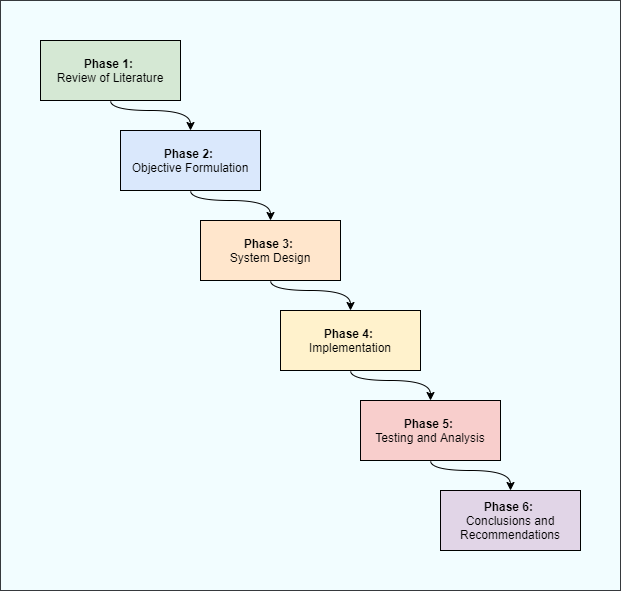
\includegraphics[width=0.7\textwidth]{figures/waterfall.png}
\caption{Project phase breakdown}
\label{fig:phase_breakdown}
\end{figure}


The rigidity of this type of developmental strategy has a number of advantages and disadvantages which will need to be considered while implementing it. The most valuable advantage of this method is the simplicity and specificity of its different phases. Each phase has set objectives to be accomplished and, once they have been achieved, the next phase begins.  It also means that the product testing does not require revisiting the implementation, allowing for well documented and coherent results. However, the rigidity of the Waterfall Method does come with shortcomings which make it non-ideal for certain types of projects. Since the implementation is started late in the developmental cycle, it is unlikely that quality of the design can be verified until it may be too late. The lack of design iteration during the implementation phase also makes it difficult to gather information about what implementing the design may entail, which will stunt the design phase. Luckily, due to this project’s clearly designed objective, the disadvantages posed by the Waterfall Design Method are unlikely to hamper the projects development. 

\section{Project Requirements}
The project requirements are the minimum nessesary criterion for which the deliverable can be described as a successful implementation. Likewise, completion of these requirements are nessesary for this deliverable to be able to undergo sufficient testing. 

\begin{enumerate}
    \item For the PEEPS application environment to be considered testable, it should:
    \begin{enumerate}
        \item contain a smartphone application that can be installed on the latest version of its relevant operating system,
        \item implement a database structure that will be used to store user and location data,
        \item provide server software that will act as an intermediary between the user and the database.
    \end{enumerate}
    \item For the PEEPS smartphone application to be considered testable it should:
    \begin{enumerate}
        \item allow users to create accounts and log into the application to ensure user data security and privacy,
        \item allow the user to select a geographical location and the application will then provide relevant information about the population statistics of that location,
        \item routinely upload the user’s geographical coordinates to a server so that it can provide population data about the user’s location to other application users.
    \end{enumerate}
    \item For the PEEPS database to be considered testable it should:
    \begin{enumerate}
        \item implement a table which stores users’ login details,
        \item implement a table which stores users’ login details,
    \end{enumerate}
    \item For the PEEPS web interface to be considered testable, it should:
    \begin{enumerate}
        \item be able to receive user data from the smartphone application and forward it to a local database,
        \item ensure user-data and database fidelity.
    \end{enumerate}
\end{enumerate}

\section{Project Constraints}
Due to the application being developed during the COVID-19 pandemic, the list of constraints reflect the necessity to mitigate the chance of infection from interactions with potentially infected individuals. While these constraints do hamper the ability of the application to undergo user testing, due to the investigative nature of the project and its reliance on software, this will not affect the ability of the PEEPS Framework to undergo thorough technical testing. The list of constraints is as follows:

\begin{itemize}
    \item Zero reliance on physical components besides the computing devices used to run the software.
    \item Zero tests of the application framework involving non-developers.
    \item Number of instances of the app being run limited by smartphone availability to researchers.
    \item An internet connection will be required for the application to perform.
\end{itemize}

\section{Technical Specifications}
These technical specifications detail the more specific aspects of the deliverable and, while not nessesary for the project to undergo testing, are what this project aims to deliver.

\subsubsection{Mobile Application Specifications}

\begin{SA}
    \item General Specifications
    \begin{SA}
        \item App must be able to run on any version of android between 6 and 10.
    \end{SA}
    \item Graphical User Interface
    \begin{SA}
        \item Must follow a consistent colour pallet with a primary and secondary colour selection.
        \item All user interactions with the app must be clearly interpretable from the GUI.
        \item Buttons must be placed below text inputs in each activity or on the toolbar.
    \end{SA}
    \item Location Services
    \begin{SA}
        \item Location must be uploaded to server at regular intervals.
        \item Location upload interval must be shorter than 20 minutes.
        \item Location data is uploaded when app in minimised.
        \item Location data is uploaded when app is closed.
        \item Location data upload starts on smartphone boot if user has logged in previously.   
    \end{SA}
    \item User interaction
    \begin{SA}
        \item User will be able to save ‘favourite’ locations by entering their coordinates.
        \item Saved locations will be stored locally using an SQL database.
        \item Saved locations will display current population density status on the app’s main page.
        \item When selected, saved locations will display a graph showing the level of activity at that location for that day, as well as the predicted activity for the rest of the day.
    \end{SA}
    \item Data security
    \begin{SA}
        \item User will need to login with correct username and password to access application.
        \item No population density data displayed on the app will contain information about the user who uploaded it.
    \end{SA}
\end{SA}

\subsubsection{Database Specifications}

\begin{SA}
    \item General Specifications
    \begin{SA}
        \item Database will be secured with appropriate password.
    \end{SA}
    \item Tables
    \begin{SA}
        \item Database will contain a table storing users’ login data.
        \item Database will contain a table storing users’ geographical data.
        \item Location table will require timestamps for each location stored and well as the username of the user who uploaded it.
    \end{SA}
\end{SA}

\subsubsection{Web Interface Specifications}

\begin{SA}
    \item General Specifications
    \begin{SA}
        \item Server is accessible from devices outside its home network.
    \end{SA}
    \item Data Communication
    \begin{SA}
        \item User and geographical data sent to the server must be checked for database compatibility.
        \item Data sent to the server, if valid, will be stored on the connected database.
        \item All location data processing will be done by the server, and only results will be forwarded to the application.
    \end{SA}
    \item Security
    \begin{SA}
        \item Data retrieved by the app from other users via the server must be anonymous.
    \end{SA}
\end{SA}